\documentclass[12pt]{article}

\usepackage{listings}
\lstset{
  language=Python
}

\usepackage{graphicx}
\graphicspath{ {../resources/feature-extraction/} }

\usepackage[margin=1in]{geometry}

\usepackage[colorlinks]{hyperref}
\hypersetup{
  urlcolor = {cyan}
}

\title{Hack the North Part 2 - Feature Extraction}
\author{Rushi Shah}
\date{19 September 2015}

\begin{document}

  \maketitle

%feature extraction picture
\begin{center}
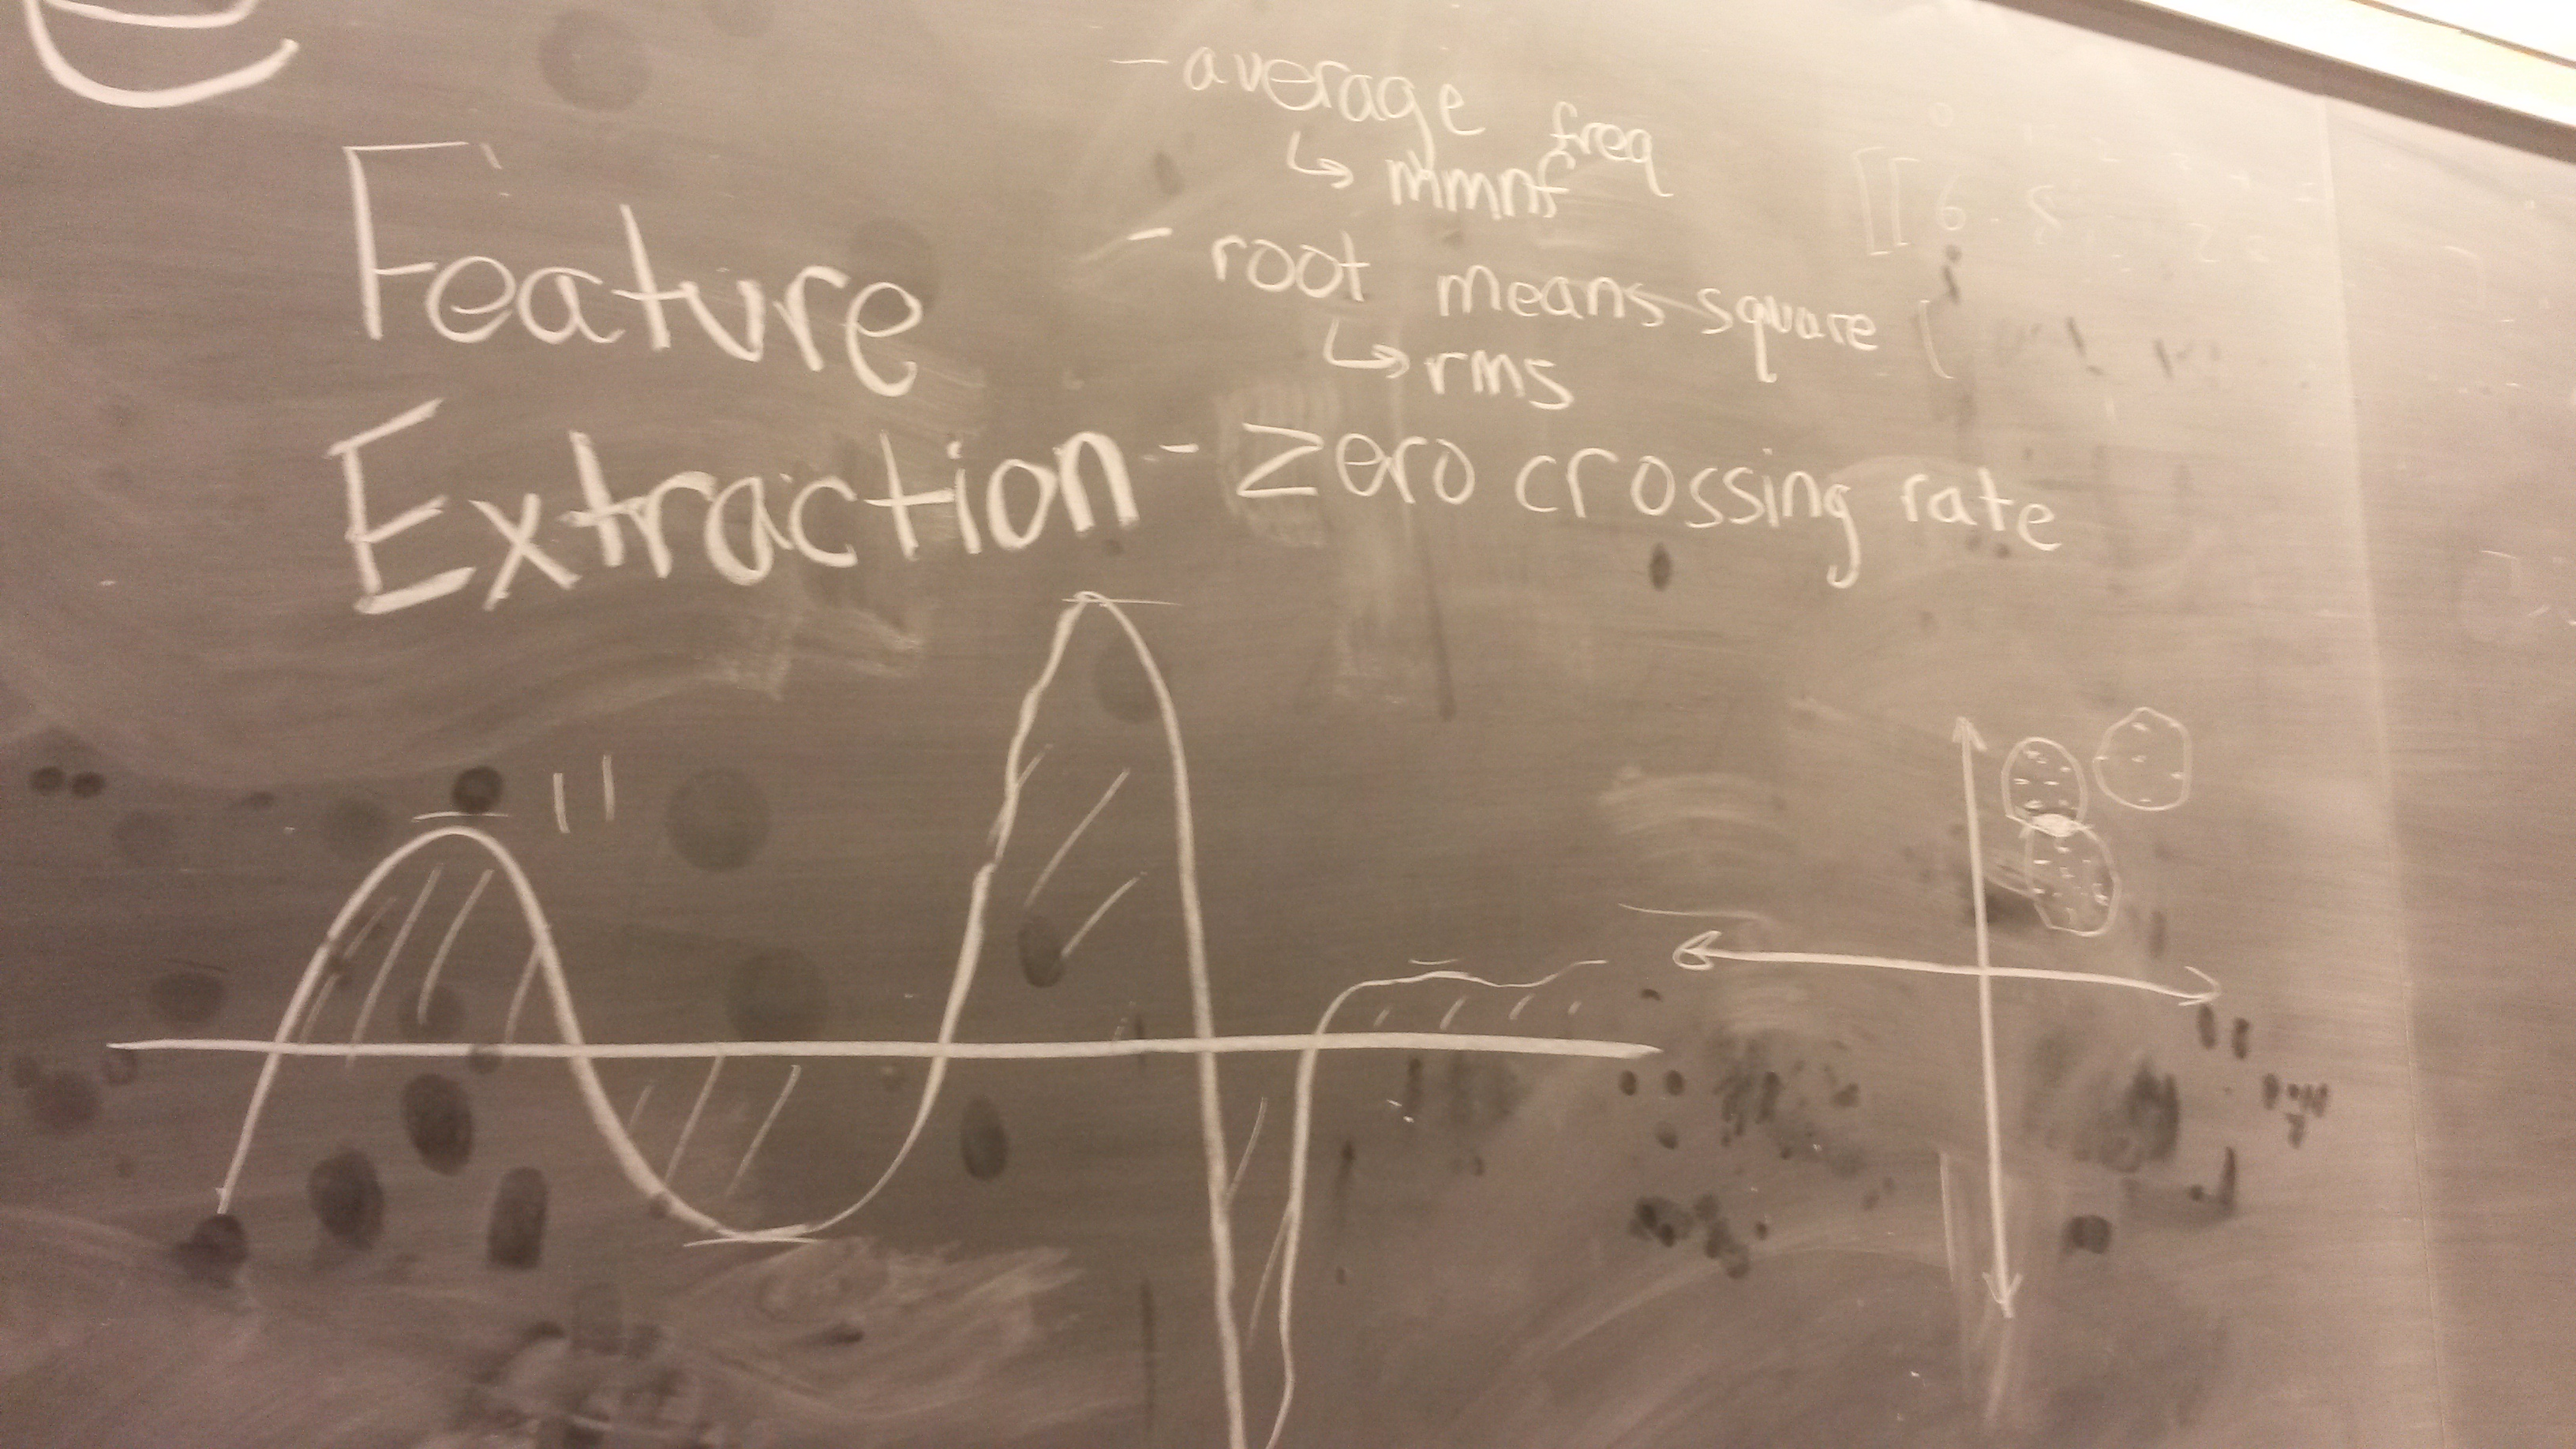
\includegraphics[width=6in]{feature-vectors}
\end{center}

So what is feature extraction? Basically, you want to take a curve and
represent the entire curve as one value. That value is called the
feature. We needed to do this at Hack the North because we wanted to
compare the output of a sensor with past data to classify it. It is
harder to compare two curves than it is to compare two values, and thus
we just treated the curves as their extracted feature and compared the
features. How might one extract a feature from a curve, you ask?

\section{Options}\label{options}

\begin{itemize}
\item
  Root mean square (RMS): square every value (to make sure everything is
  positive), then calculate the mean of the list, and calculate the
  square root (to undo the initial squaring).
\item
  Mean Absolute Value (MAV): similar to RMS, this just takes the mean
  absolute value of the list rather than squaring square-rooting every
  element
\item
  Zero crossing rate: represent the curve as the number of times it
  crosses the x-axis
\item
  Slope sign change (SSC): basically the zero crossing rate of the
  derivative of a curve made by the list values.
\item
  Integral: the area between the curve and the x-axis
\end{itemize}

\section{What we needed}\label{what-we-needed}

After analyzing some previous literature
(\href{http://wiki.epfl.ch/edicpublic/documents/Candidacy\%20exam/Zhang\%20X.\%20et\%20al.\%20(2011)\%20-\%20A\%20Framework\%20for\%20Hand\%20Gesture\%20Recognition\%20Based\%20on\%20Accelerometer\%20and\%20EMG\%20Sensors.pdf}{1}
and \href{http://rspublication.com/ijca/april13/3.pdf}{2}) we decided to
use the RMS method because of it's past successes, ease of
implementation, and relevance to the Myo data.

The Myo itself will provide us with eight sensors worth of data. Each
sensor provides it's own curve that we want to extract a feature from.
Thus given an array of eight arrays (which contain data points that
represent a curve), we need to return an array of eight number values
(eight features).

\section{Implementation}\label{implementation}

For all you imperative programmers out there, this just screams for
loop, right? Well old habits die hard so initially I whipped this simple
implementation up:

\begin{lstlisting} 
import numpy as np 
def extractFeatures(arr):
  res = [] 
  for x in arr:
    res.push(np.sqrt(np.average(np.square(np.array(x))))) 
  return res
\end{lstlisting}

But at this point in the hackathon, I had been using Haskell for the
whole weekend, so I improved it by mapping an \texttt{rms} function on
each sensor's curve:

\begin{lstlisting}  
import numpy as np 
def rms(arr): 
  return np.sqrt(np.average(np.square(np.array(arr)))) 
def extractFeatures(arr):
  # list because http://stackoverflow.com/a/1303354/3861396 
  return list(map(rms, arr)) 
\end{lstlisting} 

That's really all we needed as far as Feature Extraction goes. With that
being said, I stumbled on some very intriguing papers while researching
so if you're interested, check them out.
\href{http://wiki.epfl.ch/edicpublic/documents/Candidacy\%20exam/Zhang\%20X.\%20et\%20al.\%20(2011)\%20-\%20A\%20Framework\%20for\%20Hand\%20Gesture\%20Recognition\%20Based\%20on\%20Accelerometer\%20and\%20EMG\%20Sensors.pdf}{This
one} outlines an experiment on user-independent and user-specific EMG
Hand Gesture recognition for solving virtual Rubik's Cubes.
\href{http://rspublication.com/ijca/april13/3.pdf}{This one} gives a
nice overview of the different types of Feature Extractions like
\texttt{SSC} and \texttt{MAV}.

\end{document}
